%----------------------------------------------------------------------------------------
%	CHAPTER - INTRODUCTUION
%----------------------------------------------------------------------------------------

\chapter{Introduction} % Main chapter title

\label{ChapterIntroduction}

Technological advancements are of constant nature to us and affect most areas in our lifes. Just twenty years ago, one had to go to a physical branch of a bank to make a simple payment or check the current account balance. Then online banking emerged, soon followed by mobile banking, and the next big advancement might just be waiting ahead of us. This master thesis provides an overview of the current state of research regarding the interaction with, and visualisation of, categorized financial data in virtual reality with the intention to make exploratory analysis more simple and to provide better insights into trends and changes.

With the public release of the Oculus Rift in March 2016 \citep{Oculus2016} and the HTC Vive in April 2016 \citep{Htcvive2016}, \gls{vr} has arrived at the consumer level and is all over the news. Although we only see the first iteration of consumer products, \cite{Gartner2015} predicts that within the next five to ten years, virtual reality will achieve mainstream adoption and enter the so called "Plateau of Productivity". Gesture Control is even a bit ahead of \gls{vr} and its mainstream adoption is already expected in the next two to five years \citep{Gartner2015}. Together with the new \gls{hmd}, also the ways to interact with the virtual world have been massively improved, such as very accurate gesture controllers or full 360° motion tracking, which all are just becoming part of research now. Since these big advancements in hardware happened only very recently, the software part first has to catch up with all the new possibilities that became available. It became very easy to create 3D visualisations, but the big questions remains about why we should do that. \cite{Ware2012} sees clear clear advantages in the conventional two-dimensional techniques with bar charts and scatter plots, since the powerful pattern-finding mechanism of our brain also works in 2D. Furthermore, there are well established and effective (2D) data representations that are also very easy to be included in any kind of two-dimensional medium such as a book or a report \citep{Ware2012}. On the other side, \cite{Ware2012} also points out that we live in a three-dimensional word and interact with it so frequently that our brains got very much used to it. It is also important to understand that ultimately a 2D space is part of 3D space and thus any 2D object can always be flattened out and presented as such in 3D space. This however does not mean, that this always is a good idea. \cite{Kwon2015} stated that in a 2D environment/space (like a regular screen) it makes sense to use 2D objects for the presentation, whereas in a \gls{vr} environment where the viewing direction can be freely chosen by the user, the whole three dimensional space should be utilized. It generally can be said that we are only at the beginning of understanding how to effectively use these new means. Chapter \ref{SectionLiteratureReviewSRQ1} and \ref{SectionLiteratureReviewSRQ2} in the literature review will further discuss these new possibilities.

Simultaneously, we see massive advancements in the functionalities provided by banks to their clients. Contact-less payments and mobile banking are on the rise, and in 2014 UBS AG even won the "Master of Swiss Web" award and two gold medals for their new e-banking platform \citep{UBSAG2014}. But when clients want to look at the financial situation, nothing has changed for a long time in terms of how it is presented to the users: always the same old bar- and pie charts. Figure \ref{fig:ubsspendinganalysis} gives an impression of how exemplary data is visualized on a 2D screen. Many challenges and requirements have to be covered nowadays. Clients want to immediately see and understand their financial situation, they want to be able to make comparisons and see trends. This exploratory analysis is currently only possible with limitations, also due to the restriction of only two (real) axis that are possible on a display. \cite{Jamieson2007} see that it becomes increasingly difficult to get a meaningful understanding of the big amount of data that is still presented with traditional methods. They continue that these methods will sooner or later come to their limits and new visualisation methods have to be established \citep{Jamieson2007}. Chapter \ref{SectionLiteratureReviewSRQ3} in the literature review addresses the currently researched methods for data visualization in more detail.
\begin{figure}[h]
	\begin{center}
		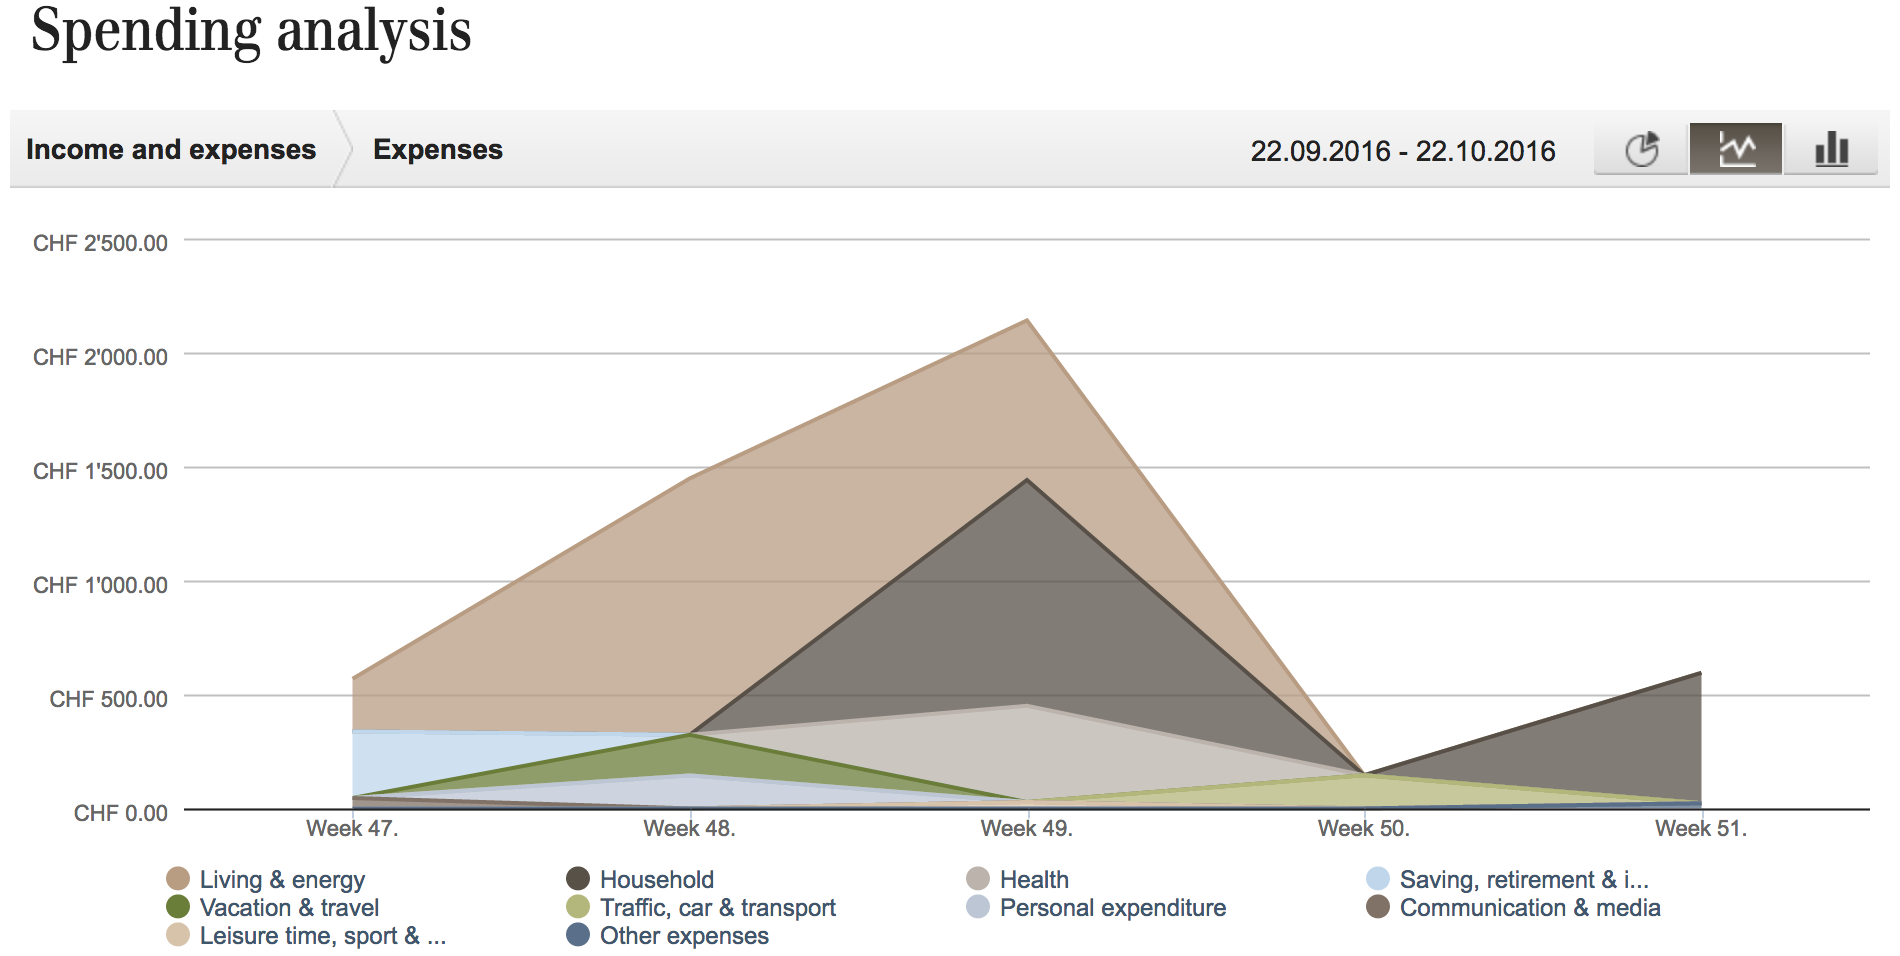
\includegraphics[width=7cm]{03_Figures/06_Introduction/UBSAG2016_SpendingAnalysis2.png}
		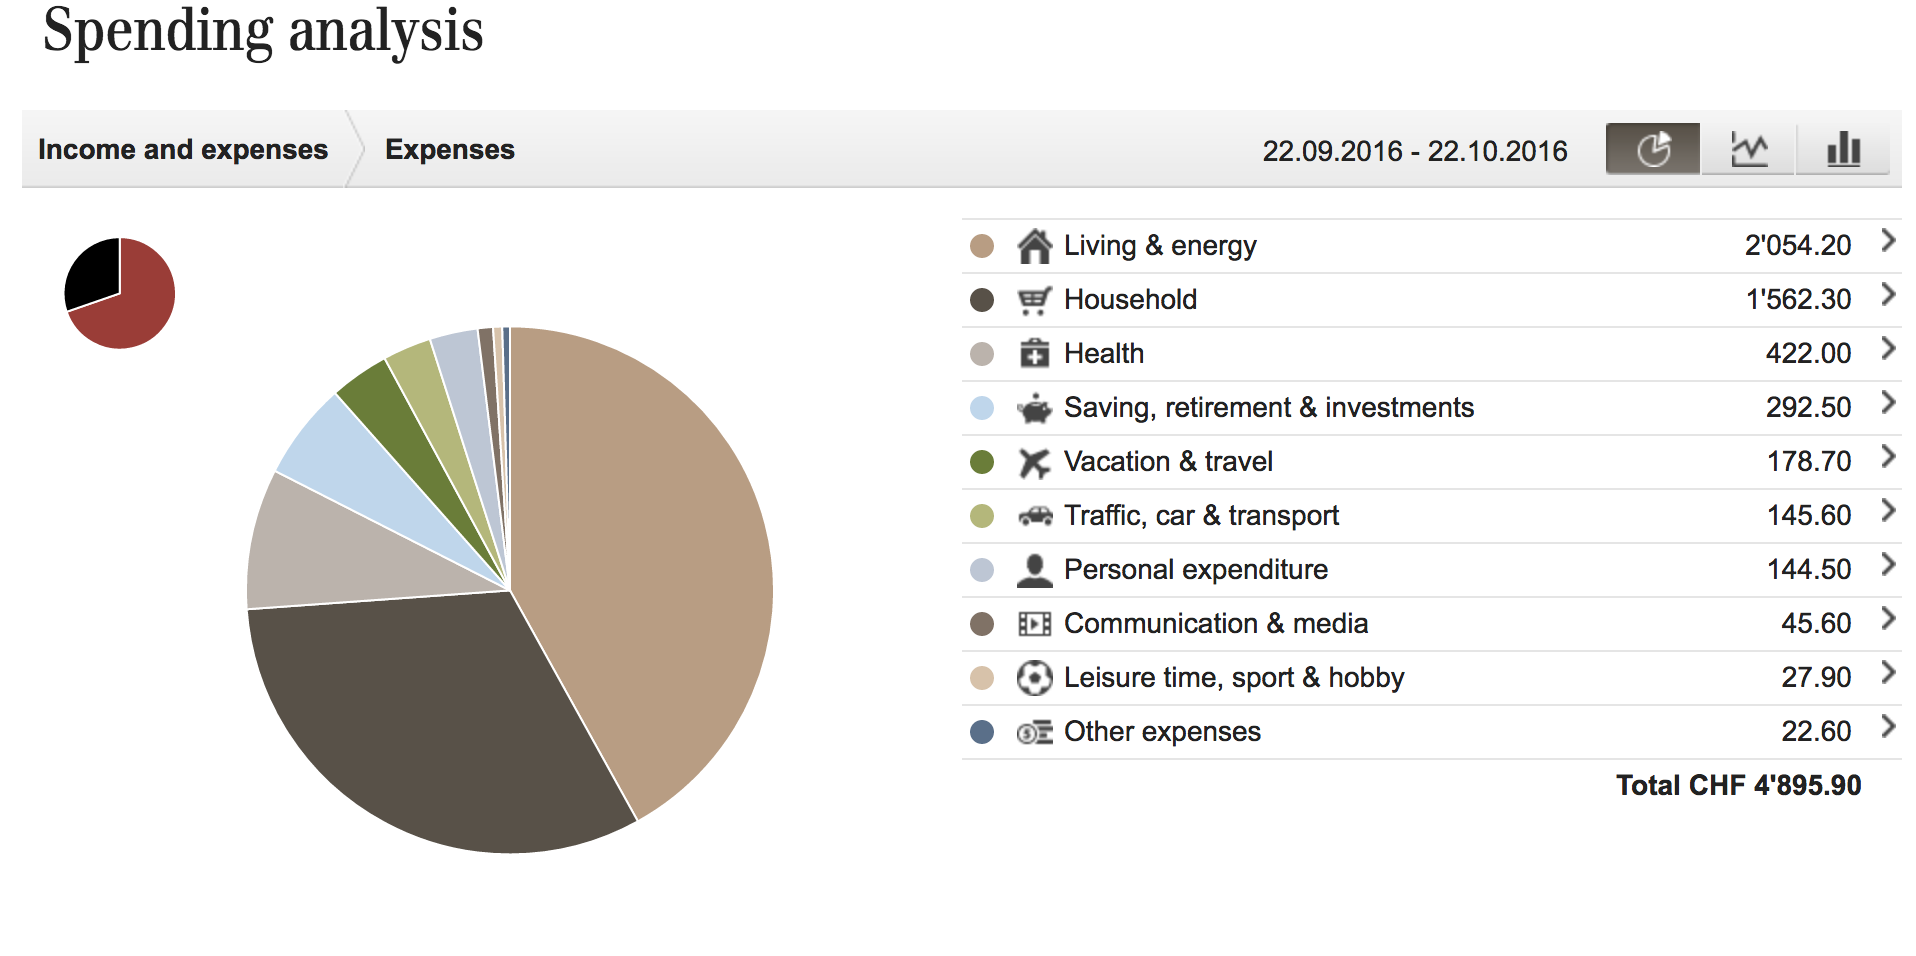
\includegraphics[width=7cm]{03_Figures/06_Introduction/UBSAG2016_SpendingAnalysis.png}
		\caption[Different visualisations of the spending analysis in UBS e-banking demo]{Different visualisations of the spending analysis in UBS e-banking demo \citep{UBSAG2016}}
		\label{fig:ubsspendinganalysis}
	\end{center}
\end{figure}

The focus of this master thesis is on the new possibilities of visualising and interacting with data about our financial situation in \gls{vr} by utilizing the latest available (consumer) \gls{vr}-hardware and research about data visualisation. The anonymized base data set of categorized financial data is shown in Appendix \ref{AppendixA} and contains detailed information about financial transactions of a single year. Not only does it contain data about the date, the currency and amount, or the recipient but every single transaction is also categorized in: \textit{Main category} and \textit{Subcategory}. A complete overview and mapping of these categories is shown below in Table \ref{tbl:financialcategories}.
\begin{longtable}{ | p{5cm} | p{9cm} |}
	\hline
	\textbf{Main category} & \textbf{Subcategory} \\
	\hline
	\endfirsthead % Line(s) to appear as head of the table on the first page
	\multicolumn{2}{c}%
	{\tablename\ \thetable\ -- \textit{Continued from previous page}} \\
	\hline
	\textbf{Main category} & \textbf{Subcategory} \\
	\hline
	\endhead % Line(s) to appear at top of every page (except first)
	\hline
	\multicolumn{2}{r}{\textit{Continued on next page}} \\
	\endfoot % Last line(s) to appear at the bottom of every page (except last)
	\endlastfoot % Last line(s) to appear at the end of the table
	\hline
	Communication \& media &
	- Film, photo, electronic devices and accessories \newline
	- Miscellaneous \newline
	- Multimedia (music, video \& apps) \newline
	- Newspaper and magazine subscriptions \newline
	- Radio and television fees \newline
	- Software \newline
	- Telephone,  Internet and TV \\
	\hline
	Health &
	- Medical services \\
	\hline
	Household &
	- Children and family \newline
	- Food and beverage \newline
	- Household articles and accessories \newline
	- Household equipment \newline
	- Office articles and services \newline
	- Pets \\
	\hline
	Income \& credits &
	- Capital revenues (interest, dividends \& earnings) \newline
	- Gifts and inheritance \newline
	- Refunds \newline
	- Salary and sideline \newline
	- Sale of property \\
	\hline
	Leisure time, sport \& hobby &
	- Books and literature \newline
	- Going out, culture and cinema \newline
	- Miscellaneous \newline
	- Toys and hobby articles \\
	\hline
	Living \& energy &
	- Building and property insurance \newline
	- Electricity and gas \newline
	- Rent and mortgage interest \newline
	- Tools and garden \\
	\hline
	Other expenses &
	- Banking services and charges \newline
	- Benefactor contributions \newline
	- Credit card invoice and fees \newline
	- Loan and debt interest \newline
	- Miscellaneous \newline
	- Repayments \\
	\hline
	Personal expenditure &
	- Clothing, shoes and accessories \newline
	- Donations \newline
	- Food (snacks, restaurants and bars) \newline
	- Gifts \newline
	- Miscellaneous \newline
	- Personal hygiene and wellness \newline
	- Training and further education \\
	\hline
	Taxes \& duties &
	- Community and cantonal tax \newline
	- Federal tax \newline
	- Fees \newline
	- Military exemption tax \\
	\hline
	Traffic, car \& transport &
	- Fuel (gasoline, diesel, gas) \newline
	- Public transport (tickets \& subscriptions) \newline
	- Traffic charges \\
	\hline
	Vacation \& travel &
	- Accommodation and hotels \newline
	- Miscellaneous \newline
	- Offers and services \newline
	- Travel and flight costs \\
	\hline
	Withdrawals &
	- Bancomat \newline
	- Teller (branch) \\
	\hline
	\caption{Mapping of Main category and Subcategory of financial data set}
	\label{tbl:financialcategories}
\end{longtable}

Due to the complexity of the data-set and the numerous different (sub-)categories, it can become difficult to keep a good overview, especially when the comparison goes across multiple months for various categories.

In the following sub-chapters, more background information about the topic is given as well as the definition of the problem statement. Based on this, the thesis statement is proposed and research questions are derived from. Following these, the delineations and limitations are presented before this chapter is closed with the structure of the thesis and a brief overview of the chapters and their correlations.


%----------------------------------------------------------------------------------------
%	SECTION 1
%----------------------------------------------------------------------------------------

\section{Background}

\gls{vr} has been around us for a few decades already, but only in the last couple of years with increasingly fast hardware and reduced costs, \gls{vr} made rapid advancements \citep{vrs2015}. Computers and even smartphones are now powerful enough to provide good \gls{vr} experiences.\newline
Very dominant at the moment are the entertainment purposes, for which \gls{vr} is currently mainly utilized, but it can also go beyond that and provide profound educational experiences if curated with the right content \citep{Safrudin2015}. \gls{vr} even should be seen as disruptive, as a \textbf{game changer} that can become accessible to everyone and will be very promising for high-tech enterprises that focus on retail and banking \citep{Safrudin2015}. \newline
Every year, Gartner publishes their hype cycle on different topics, including the \textit{Emerging Technology Hype Cycle} from 2015 (Figure \ref{fig:hypecycle}). This shows that if Gartner is to be believed, \gls{vr} has the phase of over-excitement and unrealistic expectations already behind it and is close to the point where it is widely understood by the general public. A bit further than \gls{vr} itself is Gesture Control that according to \cite{Gartner2015} will already reach mainstream adoption in the next two to five years.
\begin{figure}[h]
	\begin{center}
		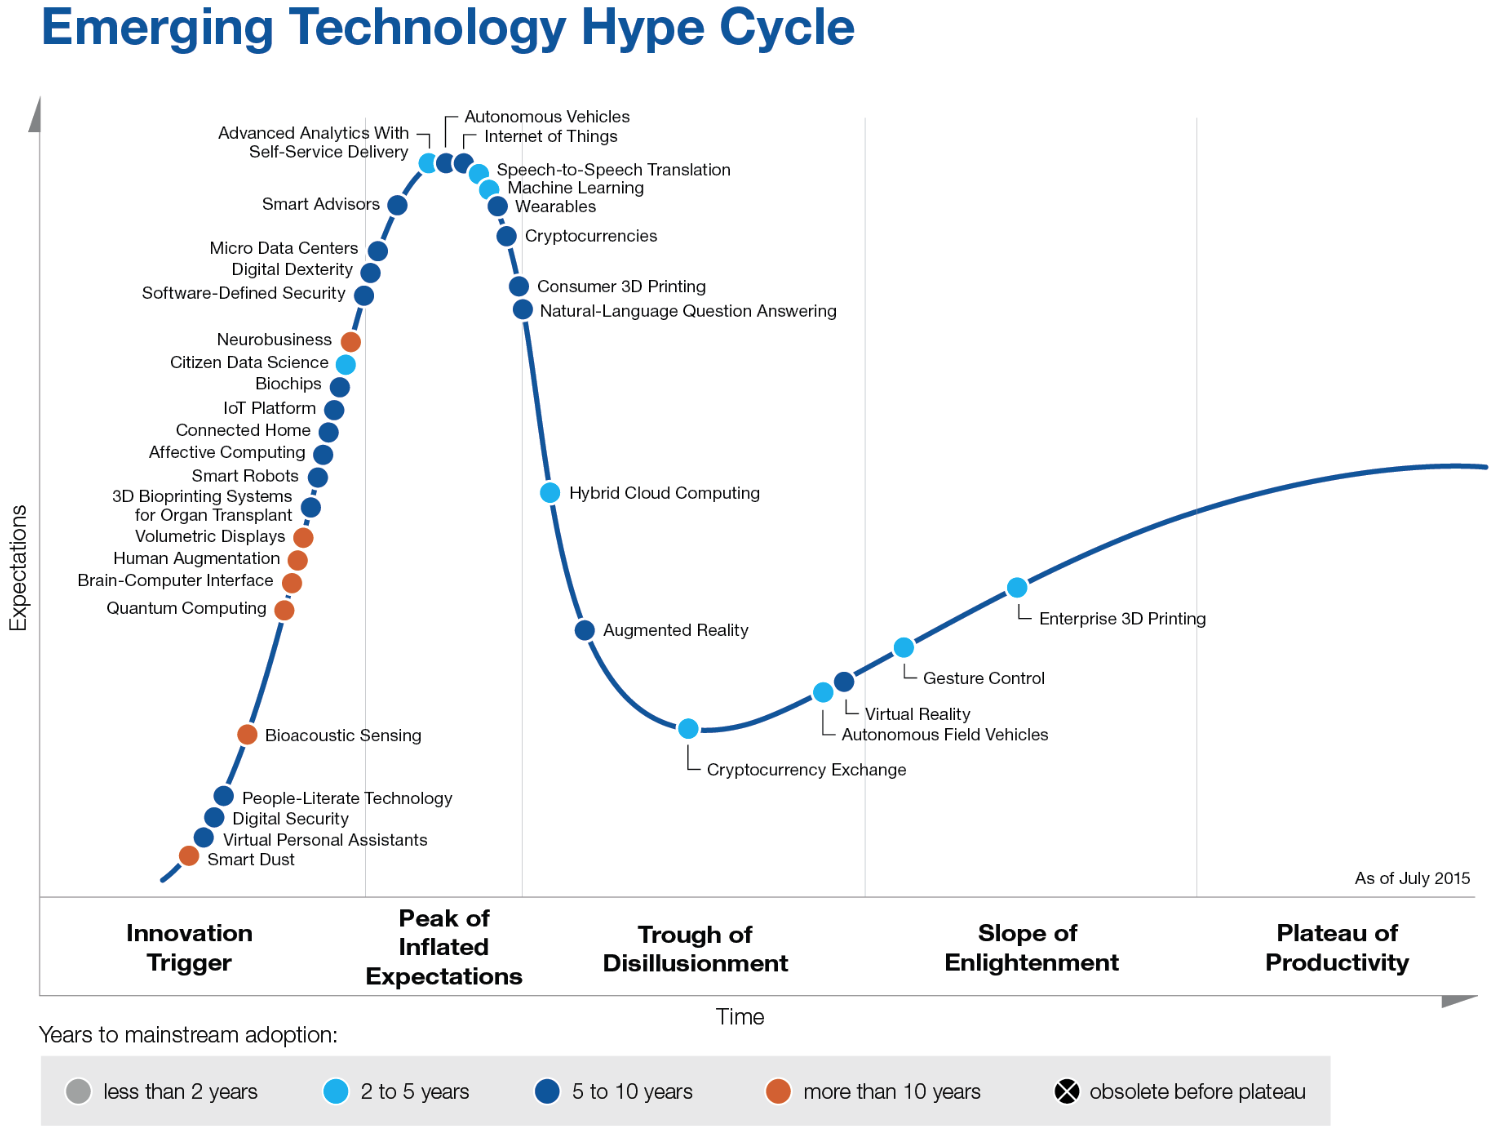
\includegraphics[width=14cm]{03_Figures/03_Gartner/Gartner_EmergingTech2015.png}
		\caption[Emerging Technology Hype Cycle]{Emerging Technology Hype Cycle \citep{Gartner2015b}}
		\label{fig:hypecycle}
	\end{center}
\end{figure} \newline
There are different interaction methods (i.e. devices to interact with the \gls{ve}) that each provide advantages and disadvantages in the execution of tasks belonging to one of three groups of interaction patterns: \textit{Travel}, \textit{Selection} and \textit{Manipulation} \citep{Bowman2002}. 


%----------------------------------------------------------------------------------------
%	SECTION 2
%----------------------------------------------------------------------------------------

\section{Problem Statement}

\gls{vr} becomes more important in our lives in the future and it is crucial to have effective and efficient means to interact with the \gls{ve} in order to secure the success of this technology. Research has been done on how to travel within the \gls{ve} and how to select objects, but not much has been done yet on the side of manipulation. While there are some guidelines and recommendations, they are all of theoretical nature and no practical recommendations for specific technologies are available. \newline
Even in 2016, the visualisation of data in a nutshell is still looking the same like a decade ago. There were only minor advancements that all are still focusing on the (limited) 2D space while only little research has been made in how to utilize the (real) third dimension in \gls{vr}.


%----------------------------------------------------------------------------------------
%	SECTION 3
%----------------------------------------------------------------------------------------

\section{Thesis Statement}

%Definition of the Thesis Statement
\newcommand{\thesisstatementtext}{Exploratory analysis of categorized financial data can be enhanced by utilizing new input methods and interaction patterns in virtual reality.}

\label{TS}

The thesis statement is as follows:
\begin{framed}
	\textit{\thesisstatementtext}
\end{framed}

%----------------------------------------------------------------------------------------
%	SECTION 4
%----------------------------------------------------------------------------------------

\section{Research question}

%Definition of the MRQ
\newcommand{\mrqtext}{How can the exploratory analysis of categorized financial data be enhanced by utilizing new input methods and interaction patterns in virtual reality?}

% Definition of the SRQs
\newcommand{\srqonetext}{Which methods of user input in virtual reality are researched and what are their advantages and disadvantages?}
\newcommand{\srqtwotext}{Which ways of interaction for multi-dimensional data exist and what are their strengths and weaknesses?}
\newcommand{\srqthreetext}{Which traditional strategies for visualization and manipulation of 2D data have been applied and enhanced for 3D space in virtual reality?}
\newcommand{\srqfourtext}{What benefits can be achieved by bringing the interaction with categorized financial into virtual reality, compared to the traditional 2D approach?}

To address the problem statement, research questions are used to break down the research into smaller parts that can be examined individually and allow a view at the nature of the problem from different perspectives. In this chapter, the \gls{mrq} as well as the \glspl{srq} are formulated. \newline
The main research question, derived from the thesis statement, is:
\begin{framed}
	\textit{\mrqtext}
\end{framed} \label{MRQ}
From the \gls{mrq}, the \glspl{srq} can be derived and are defined as follows:
\begin{framed}
	\textit{\gls{srq} 1: \srqonetext}
\end{framed} \label{SRQ1}
\begin{framed}
	\textit{\gls{srq} 2: \srqtwotext}
\end{framed} \label{SRQ2}
\begin{framed}
	\textit{\gls{srq} 3: \srqthreetext}
\end{framed} \label{SRQ3}
 \begin{framed}
 	\textit{\gls{srq} 4: \srqfourtext}
 \end{framed} \label{SRQ4}
The first three \glspl{srq} are answered as part of the literature review, whereas for \gls{srq} 4 an answer is proposed as part of the design suggestion and then validated with the implementation and evaluation of a prototype application.


%----------------------------------------------------------------------------------------
%	SECTION 5
%----------------------------------------------------------------------------------------

\section{Research Objective}

The research objective of this master thesis is to enhance the visualisation and interaction with categorized financial data in virtual reality by utilizing the latest (consumer) \gls{vr}-hardware in terms of display and input devices. \newline
This objective will be addressed by first conducting a literature review on the research that has already bee done in the fields of input methods and interaction patterns, as well as data visualisation. Based on this, a dedicated approach for the visualisation and the corresponding interaction patterns will be defined and applied in a prototype application. This also acts as a verification that the visualisation approach and interaction patterns indeed are feasible.


%----------------------------------------------------------------------------------------
%	SECTION 6
%----------------------------------------------------------------------------------------

% \section{Short Overview}


%----------------------------------------------------------------------------------------
%	SECTION 7
%----------------------------------------------------------------------------------------

\section{Delineations and Limitations}

TODO: Totall re-work this chapter! \newline
- consumer-available devices \newline
- no manual construction \newline
- no psychological aspects \newline
- no massive user tests \newline
- not a final product, its a prototype! \newline
- data security etc \newline


In this thesis, the focus lies on publicly available consumer \gls{vr} hardware and no own display or input devices will be developed. In regards of the design and implementation of the prototype, the artefact will be implemented in Unity3D 5.5.0 with the SteamVR framework. The decision for this framework is based on the fact that it acts as a consolidation layer for many different \gls{vr} devices (see Figure \ref{fig:steamvr}) and thus should provide the highest chance of re-usability for current and future \gls{vr} hardware. \newline
Furthermore, with the design and development of a prototype, this thesis focuses more on the technical feasibility than the psychological aspects of usability, user experience, or productivity measurements. 
\begin{figure}[h]
	\begin{center}
		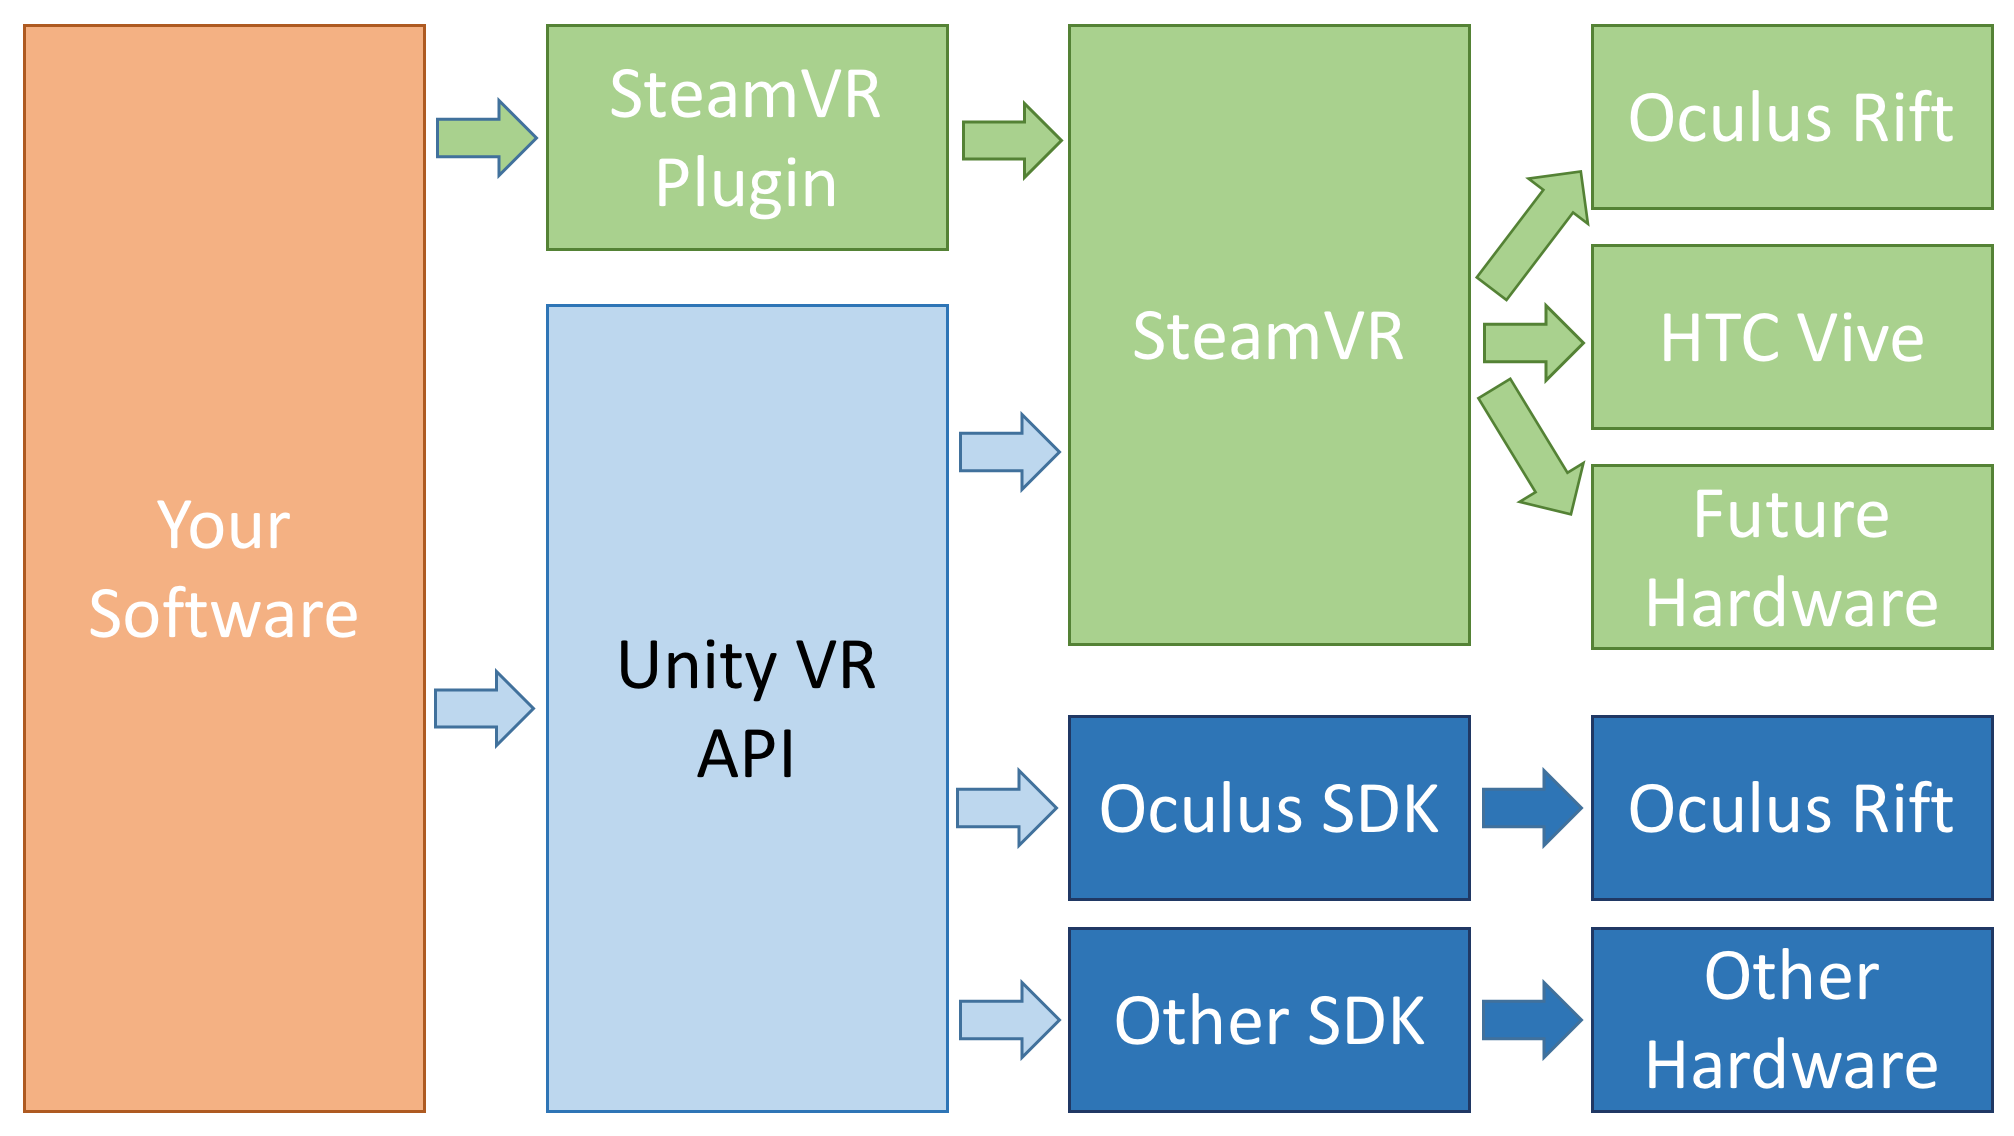
\includegraphics[width=14cm]{03_Figures/04_Valve/OpenVR_SteamVR.png}
		\caption[Steam VR Unity Plugin]{Steam VR Unity Plugin (adopted from \cite{Valve2016})}
		\label{fig:steamvr}
	\end{center}
\end{figure}

TODO: double check if this really is correct here?


%----------------------------------------------------------------------------------------
%	SECTION 8
%----------------------------------------------------------------------------------------

% \section{Underlying Assumptions}


%----------------------------------------------------------------------------------------
%	SECTION 9
%----------------------------------------------------------------------------------------

% \section{Definition of terms and concepts}


%----------------------------------------------------------------------------------------
%	SECTION 10
%----------------------------------------------------------------------------------------

% \section{Significance}


%-----------------------------------
%	SUBSECTION 1
%-----------------------------------

% \subsection{Theoretical}


%-----------------------------------
%	SUBSECTION 2
%-----------------------------------

% \subsection{Practical}


%----------------------------------------------------------------------------------------
%	SECTION 11
%----------------------------------------------------------------------------------------

\section{Thesis structure and brief chapter overviews}

The thesis map in Figure \ref{fig:thesismap} shows the structure of this thesis and the relations of the individual chapters. \newline
In chapter \ref{ChapterIntroduction}, an introduction on the topic and the research problem is given. From this the thesis statement, research questions and the research objectives are derived. Following in chapter \ref{ChapterLiteratureReview} are the literature review of different methods for user input and interaction patterns in \gls{vr} as well as the enhancement of those. The research methodology follows in chapter \ref{Research Method} where the philosophy, approach and strategy are described. \newline
\begin{figure}[pt]
	\begin{center}
		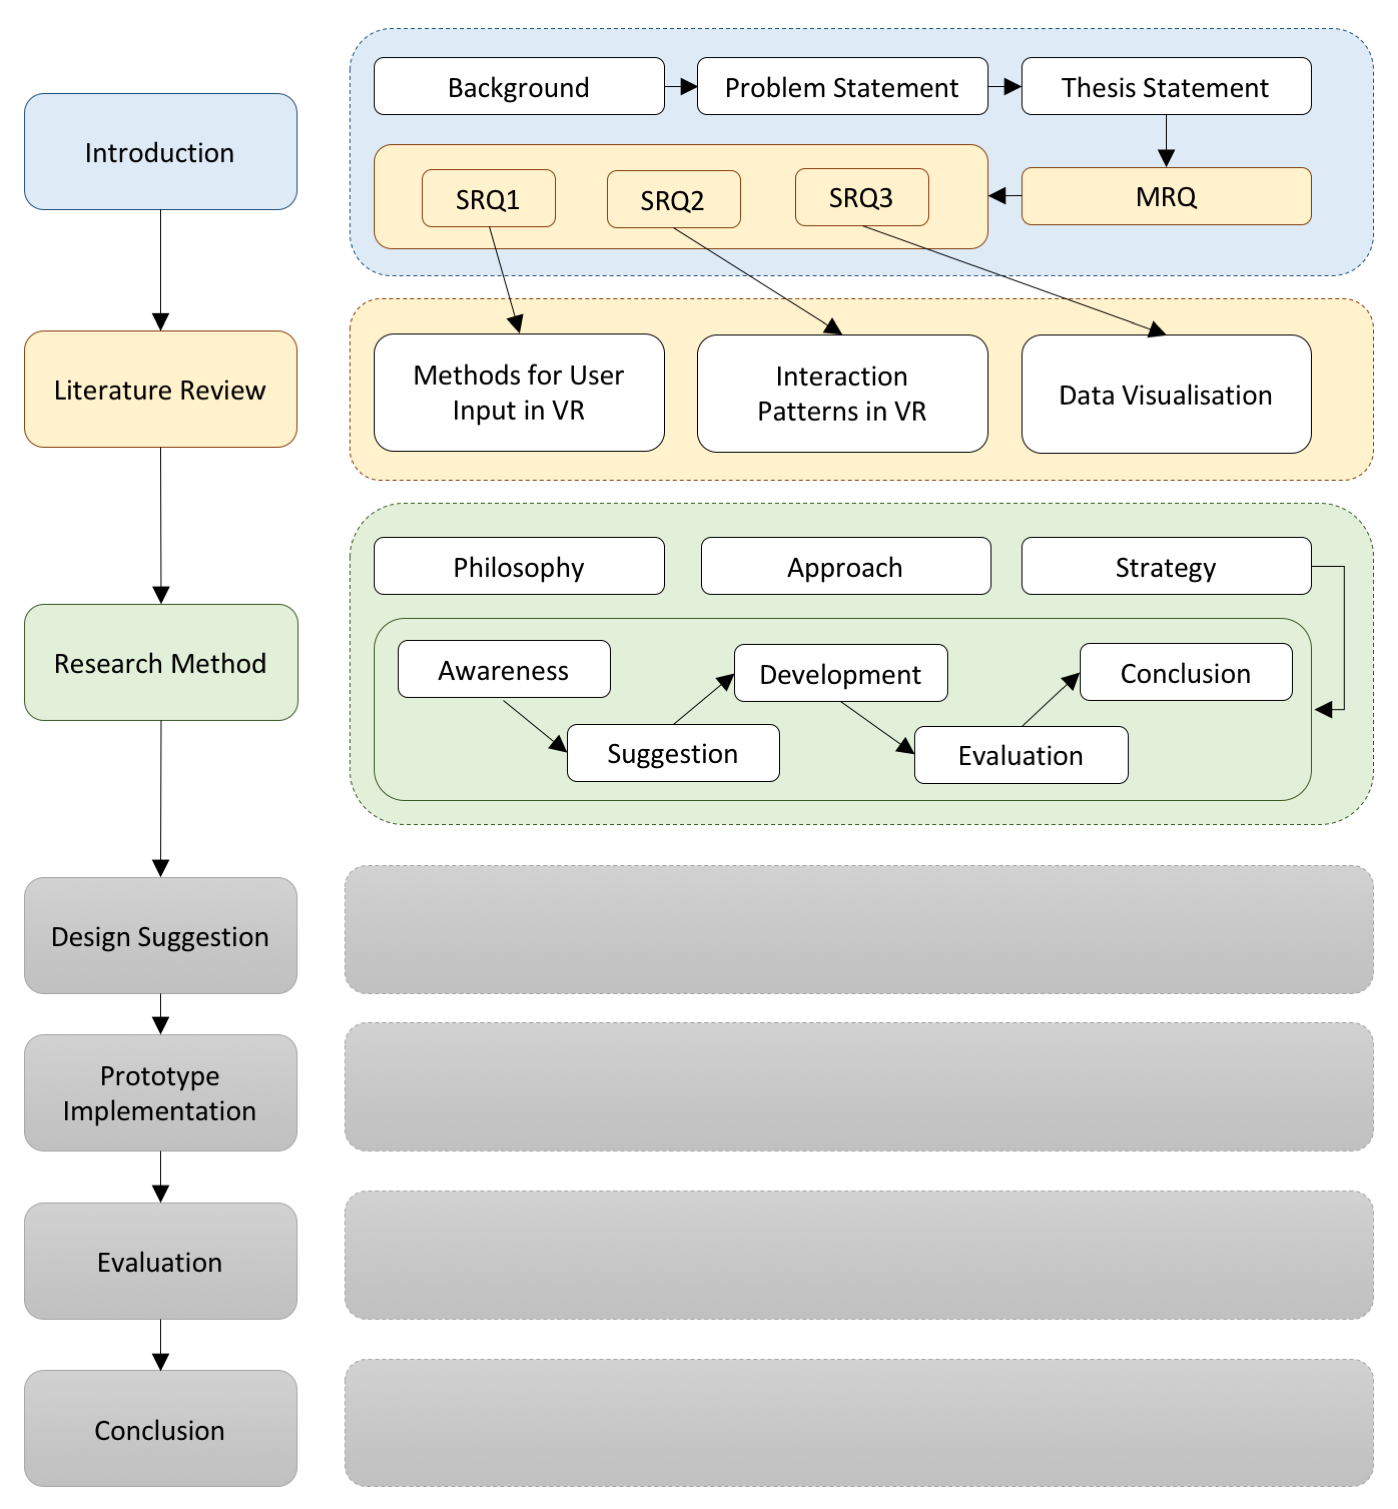
\includegraphics[width=14cm]{03_Figures/06_Introduction/ThesisMap.png}
		\caption{Thesis Map}
		\label{fig:thesismap}
	\end{center}
\end{figure}

TODO: UPDATE THIS GRAPHIC!!!

%----------------------------------------------------------------------------------------
%	SECTION 12
%----------------------------------------------------------------------------------------

% \section{Any other institutional requirement not covered here}



